Let $\bF$ be a field, and $n>0$.
We'd like to define a function which takes $n$ vectors from $\bF^n$ and computes the volume contained within them.
Since an input of $n$ vectors from $\bF^n$ is analogous to an input of a matrix from $M_n(\bF)$, by placing using the vectors as the row (or column, but here I will use row) vectors of a matrix, this defines
a function from $M_n(\bF)$ to $\bF$.
This function will be called the \emph{determinant}, denoted $\det$.
$\det$ is a function
\[ \det\colon M_n(\bF)\longto\bF \]
but since $M_n(\bF)$ is analogous to $n$ inputs of vectors in $\bF^n$, I will sometimes write $\det(v_1,\dots,v_n)$ 
So what properties should it have?

\newpage
\benum
    \item The identity matrix $I$ should have a volume of $1$ since it corresponds to the unit hypercube.
    That is, the first property is $\det(I)=1$.
    \item Let us look at the following image of some two dimensional shapes:

    \vskip12pt
    \centerline{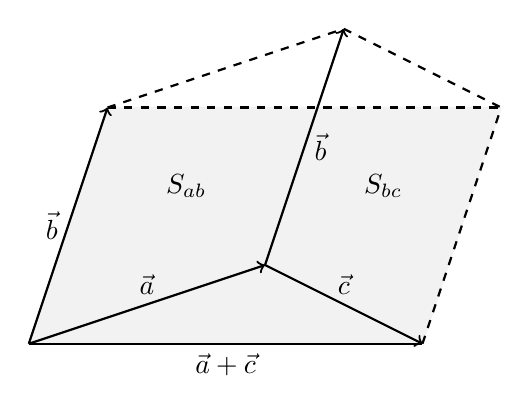
\begin{tikzpicture}
        \filldraw[color=black!5!white] (0,0) -- (5,0) -- ++(1,3) -- ++(-5,0) -- cycle;
        \draw[->, thick] (0,0) -- (3,1) node[midway, above] {$\vec a$};
        \draw[->, thick] (0,0) -- (1,3) node[midway, left] {$\vec b$};
        \draw[dashed, thick] (1,3) -- +(3,1);
        \draw[->, thick] (3,1) -- +(1,3) node[midway, right] {$\vec b$};
        \draw[->, thick] (3,1) -- (5,0) node[midway, above] {$\vec c$};
        \draw[thick] (0,0) -- (5,0) node[midway, below] {$\vec a+\vec c$};
        \draw[dashed, thick] (4,4) -- (6,3);
        \draw[dashed, thick] (5,0) -- (6,3);
        \draw[dashed, thick] (1,3) -- (6,3);
        \node at (2,2) {$S_{ab}$};
        \node at (4.5,2) {$S_{bc}$};
    \end{tikzpicture}}

    \vskip12pt
    Let $S_{ab}$ be the area contained with $\vec a$ and $\vec b$, $S_{cb}$ between $\vec c$ and $\vec b$, and $S_{(a+c)b}$ between $\vec a+\vec c$ and $\vec b$ (the grey area).
    Notice how the difference between $S_{(a+c)b}$ and $S_{ab}+S_{bc}$ is that $S_{(a+c)b}$ contains the bottom triangle, and $S_{ab}+S_{bc}$ contains the top triangle.
    But both of these triangles are defined by $\vec a$ and $\vec a+\vec c$, so they have the same area.
    Thus
    \[ S_{(a+c)b} = S_{ab} + S_{cb} \]
    Or, if we use the determinant:
    \[ \detof{\vec a+\vec c,\vec b} = \detof{\vec a,\vec b} + \detof{\vec c,\vec b} \]

    This gives us our second property: if $v_1,\dots,v_n$ are vectors in $\bF^n$, and so is $v'_i$ then
    \[ \detof{v_1,\dots,v_i+v_i',\dots,v_n} = \detof{v_1,\dots,v_i,\dots,v_n} + \detof{v_1,\dots,v'_i,\dots,v_n} \]

    \item Similar to before, if instead of adding two vectors together we scale a vector, the volume should similarly be scaled.
    In other words, if $v_1,\dots,v_n\in\bF$ and $\alpha\in\bF$ then
    \[ \detof{v_1,\dots,\alpha v_i,\dots,v_n} = \alpha\detof{v_1,\dots,v_i,\dots,v_n} \]
    This, along with the previous property, means that the determinant is linear in each component, this means the determinant is a \emph{multlinear} function.

    This property is not as innocent as it may seem.
    For example, if $\alpha=-1$, then shouldn't the determinant remain the same?
    After all, simply flipping the direction of a shape should not change its volume.
    Well, it doesn't change its volume here, rather it changes the sign of its volume.
    You could try to remedy this by scaling the determinant by $\abs\alpha$, but not every field has the notion of an absolute value, so this would be a restrictive definition.

    \item Finally, if for $i\neq j$, $v_i=v_j$ then the volume should be zero, ie.
    \[ \detof{v_1,\dots,v_n} = 0 \]
\eenum

These properties are enough to uniquely define the determinant, as we will soon show.
Suppose we have an $n\times n$ matrix $A=(a_{ij})$ (meaning the coefficient in row $i$ column $j$ is $a_{ij}$), then
\[ A = \pmat{a_{11} & \cdots & a_{1n} \\ & * &} \]
And so
\[ \det(A) = \det\pmat{a_{11}e_1 + \cdots + a_{1n}e_n \\ *} \]
Since the determinant is multilinear, this is equal to
\[ \det(A) = \sum_{i=1}^n\det\pmat{\hort & a_{1i}e_i & \hort \\ &*&} = \sum_{i=1}^n a_{1i}\det\pmat{\hort & e_i & \hort \\ &*&} \]
And we can continue this on the second row to get
\[ \detof A = \sum_{i=1}^n\sum_{j=1}^n a_{1i}a_{2j}\det\pmat{\hort & e_i & \hort \\ \hort & e_j & \hort \\ &*&} \]
Continuing, we get
\[ \detof A = \sum_{i_1=1}^n\cdots\sum_{i_n=1}^n a_{1i_1}\cdots a_{ni_n}\cdot\det\pmat{\hort & e_{i_1} & \hort \\ & \vdots & \\ \hort & e_{i_n} & \hort} \]
We can combine $i_1,\dots,i_n$ to sum over $(i_1,\dots,i_n)\in\set{1,\dots,n}^n$, which is the same as summing over functions $\sigma$ from $\set{1,\dots,n}$ to $\set{1,\dots,n}$.
Let $X$ be the set of functions from $\set{1,\dots,n}$ to $\set{1,\dots,n}$, so
\[ \detof A = \sum_{\sigma\in X}\prod_{i=1}^n a_{i\sigma(i)}\cdot\det\pmat{\hort & e_{\sigma(1)} & \hort \\ & \vdots & \\ \hort & e_{\sigma(n)} & \hort} =
\sum_{\sigma\in X}\prod_{i=1}^n a_{i\sigma(i)}\cdot\detof{e_{\sigma(1)},\dots,e_{\sigma(n)}} \]
Now, if $\sigma$ is not injective, then there exist $i\neq j$ such that $\sigma(i)=\sigma(j)$, and so $\det(e_{\sigma(1)},\dots,e_{\sigma(n)})=0$.
So we can restrict ourselves to sum only over injective $\sigma$s, ie. $\sigma\in S_n$.
So
\[ \detof A = \sum_{\sigma\in S_n}\prod_{i=1}^n a_{i\sigma(i)}\cdot\detof{e_{\sigma(1)},\dots,e_{\sigma(n)}} \]

\hypertarget{proof:detTransposition}
Now, notice that
\[ 0 = \detof{v_1,\dots,v_i+v_j,\dots,v_i+v_j,\dots,v_n} = \detof{v_1,\dots,v_i,\dots,v_i+v_j,\dots,v_n} + \detof{v_1,\dots,v_j,\dots,v_i+v_j,\dots,v_n} \]
And since
\begin{multline*}
    \detof{v_1,\dots,v_i,\dots,v_i+v_j,\dots,v_n}=\detof{v_1,\dots,v_i,\dots,v_i,\dots,v_n} + \detof{v_1,\dots,v_i,\dots,v_j,\dots,v_n} =\\
    \detof{v_1,\dots,v_i,\dots,v_j,\dots,v_n}
\end{multline*}
we get that
\[ 0 = \detof{v_1,\dots,v_i,\dots,v_j,\dots,v_n} + \detof{v_1,\dots,v_j,\dots,v_i,\dots,v_n} \]
And so
\[ \detof{v_1,\dots,v_i,\dots,v_j,\dots,v_n} = -\detof{v_1,\dots,v_j,\dots,v_i,\dots,v_n} \]
Meaning transposing the inputs of the determinant scales it by $-1$.
So if $\tau$ is a transposition of $\set{1,\dots,n}$ then
\[ \detof{v_{\tau(1)},\dots,v_{\tau(n)}} = -\detof{v_1,\dots,v_j,\dots,v_i,\dots,v_n} \]
And since every permutation can be written as a product of transpositions (since every cycle can), if $\sigma=\tau_1\cdots\tau_m$ where $\tau_i$ is a transposition then
\[ \detof{v_{\sigma(1)},\dots,v_{\sigma(n)}} = -\detof{v_{\tau_2\cdots\tau_n(1)},\dots,v_{\tau_2\cdots\tau_m(n)}} = \cdots = (-1)^m\detof{v_1,\dots,v_n} \]
And since $\signof{\sigma}=\signof{\tau_1}\cdots\signof{\tau_m}=(-1)^m$, we have that
\[ \detof{v_{\sigma(1)},\dots,v_{\sigma(n)}} = \signof\sigma\cdot\detof{v_1,\dots,v_n} \]

And in particular,
\[ \detof{e_{\sigma(1)},\dots,e_{\sigma(n)}} = \signof\sigma\cdot\signof{e_1,\dots,e_n} = \signof\sigma\det(I) = \signof\sigma \]
Thus, we have that
\[ \detof A = \sum_{\sigma\in S_n}\signof\sigma\cdot\prod_{i=1}^n a_{i\sigma(i)} \]

\begin{defn*}

    We define the \ppemph{determinant} to be the function
    \[ \det\colon M_n(\bF)\longto\bF \]
    defined by
    \[ \detof A = \sum_{\sigma\in S_n}\signof\sigma\cdot\prod_{i=1}^n a_{i\sigma(i)} \]

\end{defn*}

Now, it is very important to understand that while we showed that if a function satisfies certain properties (multlinear, determinant of $I$ is one, determinant of a matrix with two equal rows is zero), then
it must be the determinant, we did not show that the determinant satisfies these properties.
We will spend some time now proving that the determinant does indeed satisfy these properties.

\begin{exam*}

    If $A$ is a $2\times2$ matrix, suppose
    \[ A = \pmat{a&b\\c&d} \]
    then there are only two permutations in $S_2$: $\id$ and $(1,2)$, so
    \[ \detof A = a_{11}a_{22} - a_{12}a_{21} = ad - bc \]

\end{exam*}

\begin{prop*}

    If $A$ is an upper-right triangle matrix, then its determinant is equal to the product of its diagonal.
    In other words, if
    \[ A = \pmat{a_{11} & * & * \\ & \ddots & * \\ & & a_{nn}} \]
    then
    \[ \det(A) = a_{11}\cdots a_{nn} \]

\end{prop*}

\begin{proof}

    Our goal is to show that if $\sigma\in S_n$ is not the identity, then $\prod_{i=1}^n a_{i\sigma(i)}=0$.
    This is because there must exist some $i$ such that $i>\sigma(i)$, since otherwise for every $i$, $\sigma(i)\geq i$ and so $\sigma(n)=n$, $\sigma(n-1)=n-1$, and so on, so $\sigma=\id$.
    But then $a_{i\sigma(i)}=0$, and so the product is zero as well.
    So the determinant is
    \[ \detof A = \signof\id\cdot\prod_{i=1}^n a_{i\id(i)} = \prod_{i=1}^n a_{ii}\qed \]

\end{proof}

This proves that $\detof I=1$, since $I$ is an upper-right triangle matrix, whose diagonal is just ones.

\begin{prop*}

    If two rows of $A$ are equal, then $\detof A=0$.

\end{prop*}

\begin{proof}

    Suppose $R_k(A)=R_t(A)$ for $k\neq t$, and so implicitly $n>1$.
    Let $E_n$ be the set of all even permutations in $S_n$, and $O_n$ the set of all odd permutations.
    Then
    \[ \detof A = \sum_{\sigma\in E_n}\prod_{i=1}^n a_{i\sigma(i)} - \sum_{\sigma\in O_n}\prod_{i=1}^n a_{i\sigma(i)} \]
    Notice that the map $\sigma\mapsto\sigma\cdot\pmat{k&t}$ is a bijection between $E_n$ and $O_n$, and so
    \[ \detof A = \sum_{\sigma\in E_n}\prod_{i=1}^n a_{i\sigma(i)} - \prod_{i=1}^n a_{i\sigma\parens{k\:t}(i)} \]
    Now, notice that
    \blist
        \item if $i\neq k,t$, then $\sigma\pmat{k&t}(i)=\sigma(i)$ and so $a_{i\sigma\parens{k,t}(i)}=a_{i\sigma(i)}$.
        \item if $i=k$ then $a_{i\sigma\parens{k\:t}(i)}=a_{k\sigma(t)}$, and since $R_k(A)=R_t(A)$, this is equal to $a_{t\sigma(t)}$.
        \item and similarly if $i=t$, $a_{i\sigma\parens{k\:t}(i)}=a_{k\sigma(k)}$.
    \elist
    Thus
    \[ \prod_{i=1}^n a_{i\sigma\parens{k\:t}(i)} = \prod_{i=1}^n a_{i\sigma(i)} \]
    and so $\detof A=0$ as required.
    \qed

\end{proof}

\begin{prop*}

    The determinant is multlinear.

\end{prop*}

\begin{proof}

    We will first show that multiplying a row by a scalar scales the determinant:
    \begin{multline*}
        \detof{v_1,\dots,\alpha v_i,\dots,v_n} = \sum_{\sigma\in S_n}\signof\sigma\cdot v_{1\sigma(1)}\cdots \alpha v_{i\sigma(i)}\cdots v_{n\sigma(n)} =
        \alpha\sum_{\sigma\in S_n}\signof\sigma\cdot v_{1\sigma(1)}\cdots v_{i\sigma(i)}\cdots v_{n\sigma(n)} =\\
        \alpha\detof{v_1,\dots,v_i,\dots,v_n}
    \end{multline*}
    as required.
    Next
    \begin{multline*}
        \detof{v_1,\dots,v_i+v'_i,\dots,v_n} = \sum_{\sigma\in S_n}\signof\sigma\cdot v_{1\sigma(1)}\cdots(v_{i\sigma(i)}+v'_{i\sigma(i)})\cdots v_{n\sigma(n)} =\\
        \sum_{\sigma\in S_n}\signof\sigma\cdot v_{1\sigma(1)}\cdots v_{i\sigma(i)}\cdots v_{n\sigma(n)} + \sum_{\sigma\in S_n}\signof\sigma\cdot v_{1\sigma(1)}\cdots v'_{i\sigma(i)}\cdots v_{n\sigma(n)} =\\
        \detof{v_1,\dots,v_i,\dots,v_n} + \detof{v_1,\dots,v'_i,\dots,v_n}
    \end{multline*}
    as required.
    \qed

\end{proof}

This completes the proof that the determinant satisfies the properties we layed out earlier.

Also if some row of $A$'s is zero, then $\detof A=0$ since the determinant is multlinear, and so multiplying the row by zero results in the same matrix, and so $0\cdot\detof A=\detof A$.

\begin{prop*}

    If $\rho$ is a row operation, and $A$ a matrix then
    \blist
        \item If $\rho$ corresponds to $R_i\varleftarrow R_i+\alpha R_j$ then $\detof{\rho(A)}=\detof A$.
        \item If $\rho$ corresponds to $R_i\varleftarrow \alpha R_i$ then $\detof{\rho(A)}=\alpha\detof A$.
        \item If $\rho$ corresponds to $R_i\oto R_j$ then $\detof{\rho(A)}=-\detof A$.
    \elist

\end{prop*}

\begin{proof}

    Let us assume that $i<j$ for each case.

    \blist
        \item Let $v_i$ be the $i$th row of $A$, then
        \[ \detof{\rho(A)} = \detof{v_1,\dots,v_i+\alpha v_j,\dots,v_j,\dots,v_n} = \detof{v_1,\dots,v_i,\dots,v_j,\dots,v_n} + \alpha\detof{v_1,\dots,v_j,\dots,v_j,\dots,v_n} \]
        and since the second determinant has a repeated row, it is zero, so this is equal to
        \[ = \detof{v_1,\dots,v_i,\dots,v_j,\dots,v_n} = \detof A \]
        as required.

        \item This is just scaling a row, and is due to the determinant being mutilinear.

        \item We showed \hyperlink{proof:detTransposition}{here}, when deriving the definition of the determinant, that if the determinant is multlinear and zero when there are repeated rows (which we have
        shown), that a transposition of rows results in the determinant being scaled by $-1$.
        \qed
    \elist

\end{proof}

What this means is that if $\rrefof A$ is the reduced row echelon form of $A$, then
\[ \detof{\rrefof A} = \alpha\detof A \]
for some $\alpha\neq0$.
This is because $\rrefof A$ is obtained by composing row operations, and each row operation scales $\detof A$ by some non-zero scalar.

\begin{thrm*}

    $A$ is invertible if and only if $\detof A\neq0$.

\end{thrm*}

\begin{proof}

    Recall that $A$ is invertible if and only if $\rrefof A=I$.
    Now, if $A$ is invertible then
    \[ \detof{\rrefof A} = \alpha\detof A \implies 1=\detof I=\alpha\detof A \]
    therefore $\detof A\neq0$.

    And if $A$ is singular (not invertible), then $\rrefof A$ is an upper right triangle matrix which has at least one zero on the diagonal.
    Since the determinant of an upper right triangle matrix is the product of the numbers on its diagonal, this means $\detof{\rrefof A}=0$.
    So
    \[ 0 = \alpha\detof A \implies \detof A = 0 \qed \]

\end{proof}

\begin{thrm*}

    If $A$ and $B$ are matrices then $\detof{AB}=\detof A\detof B$.

\end{thrm*}

\begin{proof}

    If $A$ is singular, then so is $AB$ and so
    \[ \detof{AB}=0,\quad \detof A\detof B = 0\detof B = 0 \]
    Otherwise, $A$ is the product of elementary matrices (matrices of the form $\rho(I)$ where $\rho$ is a row operation).
    To start, suppose $A$ is an elementary matrix, so $A=\rho(I)$ for some row operation.
    \blist
        \item If $\rho$ corresponds to $R_i\varleftarrow R_i+\alpha R_j$ then we showed $\detof A=\detof{\rho(I)}=\detof I=1$.
        And so $\detof{AB} = \detof{\rho(B)} = \detof B=\detof A\detof B$ as required.
        \item If $\rho$ corresponds to $R_i\varleftarrow \alpha R_i$ then $\detof A=\detof{\rho(I)}=\alpha\detof I=\alpha$.
        And so $\detof{AB}=\detof{\rho(B)}=\alpha\detof B=\detof A\detof B$.
        \item And if $\rho$ corresponds to $R_i\oto R_j$ then $\detof A=\detof{\rho(I)}=-\detof I$.
        And so $\detof{AB}=\detof{\rho(B)}=-\detof B=\detof A\detof B$.
    \elist
    So if $A$ is an elementary matrix then
    \[ \detof{AB} = \detof A\detof B \]

    Otherwise, $A$ is the product of elementary matrices $A=E_1\cdots E_n$.
    So
    \[ \detof{AB} = \detof{E_1\cdots E_nB} = \detof{E_1\bigl(E_2\cdots E_nB\bigr)} = \detof{E_1}\cdot\detof{E_2\cdots E_nB} = \cdots = \detof{E_1}\cdots\detof{E_n}\detof B \]
    And
    \[ \detof A=\detof{E_1\cdots E_n}=\cdots=\detof{E_1}\cdots\detof{E_n} \]
    So all in all we get that
    \[ \detof{AB} = \detof A\detof B \qed \]

\end{proof}

\begin{coro*}

    If $A$ is an invertible matrix then $\detof{A^{-1}}=\detof A^{-1}$.

\end{coro*}

This is simple, as on one hand $\detof{AA^{-1}}=\detof I=1$, while on the other hand $\detof{AA^{-1}}=\detof A\cdot\detof{A^{-1}}$, and so
\[ \detof A\cdot\detof{A^{-1}} = 1 \implies \detof{A^{-1}} = \detof A^{-1} \]

\begin{prop*}

    $\detof A=\detof{A^\top}$.

\end{prop*}

\begin{proof}

    Since $a^\top_{i\sigma(i)}=a_{\sigma(i)i}$ we have
    \[ \detof{A^\top} = \sum_{\sigma\in S_n}\signof\sigma\prod_{i=1}^n a_{\sigma(i)i} \]
    Now, we can reorder the product with the permutation $\sigma^{-1}$, and so
    \[ = \sum_{\sigma\in S_n}\signof\sigma\prod_{i=1}^n a_{i\sigma^{-1}(i)} \]
    Notice that $\signof\sigma\cdot\signof{\sigma^{-1}}=\signof{\sigma\sigma^{-1}}=1$, and so $\signof\sigma=\signof{\sigma^{-1}}$, therefore
    \[ = \sum_{\sigma\in S_n}\signof{\sigma^{-1}}\prod_{i=1}^n a_{i\sigma^{-1}(i)} \]
    This is just a reordering of the sum which defines $\detof A$, and therefore is just equal to $\detof A$.
    \qed

\end{proof}

Since column operations are equivalent to row operations on $A^\top$, if $\rho$ is a column operation then let $\rho^\top$ be its associated row operation (eg. if $\rho$ is $C_i\varleftarrow C_i+\alpha C_j$
then $\rho^\top$ is $R_i\varleftarrow R_i+\alpha R_j$).
Then $\rho(A)=\bigl(\rho^\top(A^\top)\bigr)^\top$ (perform the row operation on $A^\top$ and then take its transpose).
Therefore
\[ \detof{\rho(A)} = \detof{\bigl(\rho^\top(A^\top)\bigr)^\top} = \detof{\rho^\top(A^\top)} \]
and so if
\blist
    \item $\rho$ corresponds to $C_i\varleftarrow C_i+\alpha C_j$, $\detof{\rho^\top(A^\top)}=\detof{A^\top}=\detof A$.
    \item $\rho$ corresponds to $C_i\varleftarrow\alpha C_i$, $\detof{\rho^\top(A^\top)}=\alpha\detof{A^\top}=\alpha\detof A$.
    \item $\rho$ corresponds to $C_i\oto C_j$, $\detof{\rho^\top(A^\top)}=-\detof{A^\top}=-\detof A$.
\elist

So column operations have the same effect on the determinant as row operations.

\begin{defn*}

    Suppose $A\in M_n(\bF)$, we define $A_{ij}\in M_{n-1}(\bF)$ to be the matrix obtained by removing the $i$th row and $j$th column from $A$.
    The \ppemph{minor} defined by $i$ and $j$ is $\detof{A_{ij}}$.

\end{defn*}

This notation is a bit confusing since $A_{ij}$ is sometimes used as the coefficient in the $i$th row and $j$th column in $A$, but the meaning of $A_{ij}$ should be clear from context.

\begin{lemm*}[blockMatrixDeterminant]

    If $A$ is a matrix of the form
    \[ A = \parens{\!\!\!\begin{array}{c|c} B&C\\\hline0&D \end{array}\!\!\!} \]
    Where $B\in M_n(\bF)$ and $D\in M_m(\bF)$.
    Then $\detof A=\detof B\cdot\detof D$.

\end{lemm*}

\begin{proof}

    Let $\sigma\in S_{n+m}$, if there is some $n+1\leq i$ such that $1\leq\sigma(i)\leq n$, $a_{i\sigma(i)}=0$, and so it does not contribute to the determinant.
    Now, suppose $\sigma\in S_{n+m}$ such that $\sigma([n+1,n+m])=[n+1,n+m]$ (ie. it doesn't map $n+1\leq i$ to $1\leq\sigma(i)\leq n$, so it may contribute to the determinant), then for every
    $1\leq i\leq n$, $1\leq\sigma(i)\leq n$ (since otherwise $\sigma$ would not be injective).
    This means that for $\sigma$ to contribute, $a_{i\sigma(i)}$ is an element in $B$ or $D$, and thus if we define
    \[ \sigma_1\colon\set{1,\dots,n}\longto\set{1,\dots,n},\quad \sigma_1(i) = \sigma(i) \]
    and
    \[ \sigma_2\colon\set{1,\dots,m}\longto\set{1,\dots,m},\quad \sigma_2(i) = \sigma(i+n)-n \]
    Then $\sigma=\sigma_1\circ\sigma_2$ and so $\signof\sigma=\signof{\sigma_1}\cdot\signof{\sigma_2}$, and also note that $\sigma\mapsto(\sigma_1,\sigma_2)$ is a bijection between contributing permutations
    and $S_n\times S_m$.
    Thus
    \[ \detof A = \sum_{\sigma}\signof\sigma\cdot\prod_{i=1}^n b_{i\sigma(i)}\cdot\prod_{i=n+1}^{n+m} d_{i-n,\sigma(i-n)+n} =
    \sum_{\sigma}\signof{\sigma_1}\cdot\prod_{i=1}^n b_{i\sigma_1(i)}\cdot\prod_{i=1}^m d_{i\sigma_2(i)} \]
    (The sum is over contributing permutations.)
    Since there is a correspondence between contributing permutations and $S_n\times S_m$, this is equal to
    \[ = \sum_{\substack{\sigma_1\in S_n\\\sigma_2\in S_m}}\signof{\sigma_1}\cdot\signof{\sigma_2}\cdot\prod_{i=1}^n b_{i\sigma_1(i)}\cdot\prod_{i=1}^m d_{i\sigma_2(i)} =
    \sum_{\sigma_1\in S_n}\signof{\sigma_1}\prod_{i=1}^n b_{i\sigma_1(i)} \cdot \sum_{\sigma_2\in S_m}\signof{\sigma_2}\prod_{i=1}^m d_{i\sigma_2(i)} \]
    which is just equal to $\detof B\cdot\detof D$, as required.
    \qed

\end{proof}

\begin{thrm*}[laplaceFormula,Laplace's\ Formula\ for\ Determinants]

    Let $A$ be a matrix in $M_n(\bF)$ then for any $1\leq i\leq n$,
    \[ \detof A = \sum_{j=1}^n (-1)^{i+j} a_{ij}\cdot\detof{A_{ij}} = \sum_{j=1}^n (-1)^{i+j} a_{ji}\cdot\detof{A_{ji}} \]

\end{thrm*}

The first formula involves summing the coefficients of $A$ in the $i$th row times the minors, and the second formula involves summing over the $i$th column.

\begin{proof}

    We will first prove the first equality.
    Let $v_t$ be the $t$th row of $A$, and suppose $v_i=(a_{i1},\dots,a_{in})$ and so
    \[ \detof A = \detof{v_1,\dots,a_{i1}e_1+\cdots+a_{in}e_n,\dots,v_n} = \sum_{j=1}^n a_{ij}\detof{v_1,\dots,e_j,\dots,v_n} \]
    Our goal is to permute the inputs of the determinant to get something of the form $\detof{e_j,v_1,\dots,v_n}$.
    This corresponds to the cycle $\pmat{1&2&3&\dots&i-1&i}$ (move each vector $v_t$ for $1\leq t<i$ to the right one, and move $e_j$ to the first position).
    This has a sign of $(-1)^i$, and so
    \[ \detof{e_j,v_1,\dots,v_n} = (-1)^i\detof{v_1,\dots,e_j,\dots,v_n} \implies \detof{v_1,\dots,e_j,\dots,v_n} = (-1)^i\detof{e_j,v_1,\dots,v_n} \]
    Let us define
    \[ A_j = \pmat{\hort&e_j&\hort\\\hort&v_1&\hort\\&\vdots&\\\hort&v_n&\hort} \]
    So we have that
    \[ \detof A = \sum_{j=1}^n(-1)^ia_{ij}\detof{A_j} \]
    Now, notice that
    \[ A_j^\top = \pmat{\vert & \vert & & \vert \\ e_j & v_1 & \cdots & v_n \\ \vert & \vert & & \vert} =
    \pmat{0 & \alpha_{11} & \cdots & \alpha_{n1} \\ \vdots & \vdots & \ddots & \vdots \\
    1 & \alpha_{1j} & \cdots & \alpha_{nj} \\ \vdots & \vdots & \ddots & \vdots \\
    0 & \alpha_{1n} & \cdots & \alpha_{nn}} \]
    ($v_i$ does not appear as a column in $A_j^\top$.)
    And similar to before, by using the permutation $\pmat{1&2&\dots&j-1&j}$ on the rows $A_j^\top$, we get the matrix
    \[ \pmat{1 & \alpha_{1j} & \cdots & \alpha_{nj} \\ 0 & \alpha_{11} & \cdots & \alpha_{n1} \\ \vdots & \vdots & \ddots & \vdots \\ 0 & \alpha_{1n} & \cdots & \alpha_{nn}} =
    \pmat{
    1 & \begin{matrix}* & \cdots & *\\\hline\end{matrix} \\
    \begin{matrix}0\\\vdots\\ 0\end{matrix}\hspace\arraycolsep\vline\hspace{-\arraycolsep}& (A_{ij})^\top} \]
    Transposing this matrix gives
    \[ \pmat{
    1 & \begin{matrix}0 & \cdots & 0\\\hline\end{matrix} \\
    \begin{matrix}*\\\vdots\\ *\end{matrix}\hspace\arraycolsep\vline\hspace{-\arraycolsep}& A_{ij}} \]
    which has the same determinant.

    Since the permutation we used to get this matrix has a sign of $(-1)^j$, we have that
    \[ \detof{A_j} = \detof{A_{j}^\top} = (-1)^j\det\pmat{
    1 & \begin{matrix}0 & \cdots & 0\\\hline\end{matrix} \\
    \begin{matrix}*\\\vdots\\ *\end{matrix}\hspace\arraycolsep\vline\hspace{-\arraycolsep}& A_{ij}} = (-1)^j\detof{A_{ij}} \]
    And so finally we have that
    \[ \detof A = \sum_{j=1}^n(-1)^ia_{ij}\detof{A_j} = \sum_{j=1}^n(-1)^{i+j}a_{ij}\detof{A_{ij}} \]
    as required.

    For the second equality, this is because
    \[ \detof{A^\top} = \sum_{j=1}^n (-1)^{i+j}a^\top_{ij}\detof{(A^\top)_{ij}} = \sum_{j=1}^n (-1)^{i+j}a_{ji}\detof{A_{ji}} \]
    as required.
    \qed

\end{proof}

\begin{exam*}

    Let
    \[ A = \pmat{1 & 2 & 5 \\ 0 & 3 & 2 \\ 1 & 2 & 4} \]
    Using the definition of the determinant, we need for every $\sigma\in S_3$ to compute $a_{1\sigma(1)}\cdot a_{2\sigma(2)}\cdot a_{3\sigma(3)}$.
    Now,
    \[ \begin{array}{c|c}
    \id & 1\cdot3\cdot4=12 \\ 
    (1,2)& 2\cdot0\cdot4=0\\
    (1,3)& 5\cdot3\cdot1=15\\
    (2,3)& 1\cdot2\cdot2=4\\
    (1,2,3)& 2\cdot2\cdot1=4\\
    (1,3,2)& 5\cdot0\cdot2=0
    \end{array}
    \]
    And so
    \[ \detof A = 12 - 0 - 15 - 4 + 4 + 0 = -3 \]

    Using Laplace's formula, let us use the second formula for minors obtained from the first column:
    \[ \detof A = 1\cdot\det\pmat{3&2\\2&4} - 0\cdot\det\pmat{2&5\\2&4} + 1\cdot\det\pmat{2&5\\3&2} = 12-4 + 4-15 = -3 \]

    But recall that row operations only scale the determinant by a known constant.
    So, let us use row operations to transform $A$ into an upper right triangle matrix:
    \[ A\xvarrightarrow{R_1\oto R_3}[-1]\pmat{1 & 2 & 4 \\ 0 & 3 & 2 \\ 1 & 2 & 5}\xvarrightarrow{R_3\varleftarrow R_3-R_1}[1]\pmat{1&2&4 \\ 0&3&2 \\ 0&0&1} \]
    The determinant of this transformed matrix is the product of the numbers on its diagonal, which is $3$.
    And if you look at the values which the row operations transformed the determinant by (below the arrows), we see that the row operations scaled the determinant by $-1$, so
    \[ 3 = -\detof A \implies \detof A = -3 \]

    This gives three methods of computing the determinant of a matrix.
    The naive method (the first method) is usually never used, since it takes time to both compute the permutations and then calculate the product.
    Laplace's formula is better for matrices which have a row or column with many zeros, but in general it is no quicker than the naive computation (because the time it takes to compute is
    $T(n)=nT(n-1)$, which gives $T(n)\in\Theta(n!)$, which is the same time complexity of the naive computation).

    The third method (using row operations to reduce the matrix to an upper right triangle matrix) may be ideal if you're good at row reduction.
    We can use column operations as well as row operations to reduce the matrix if that helps.

\end{exam*}

Laplace's formula also gives us some other important results, which we will cover now.

\begin{defn*}

    Let $A\in M_n(\bF)$, then we define the \ppemph{adjugate} matrix of $A$ (also commonly called the adjoint), by
    \[ [\adjof A]_{ij} = (-1)^{i+j}\detof{A_{ji}} \]

\end{defn*}

\begin{prop*}

    $A\cdot\adjof A=\adjof A\cdot A=\detof AI$.

\end{prop*}

\begin{proof}

    We will just compute this using definitions
    \[ [A\cdot\adjof A]_{ij} = \sum_{t=1}^n [A]_{it}[\adjof A]_{tj} = \sum_{t=1}^n (-1)^{t+j}a_{it}\detof{A_{jt}} \]
    If $i=j$ then this is equal to
    \[ = \sum_{t=1}^n (-1)^{t+i}a_{it}\detof{A_{it}} = \detof A \]
    Else if $i\neq j$ then let us define the matrix $B$ such that $R_t(B)=R_t(A)$ for $t\neq j$ and $R_j(B)=R_i(A)$.
    Then using Laplace's formula on the $j$th row, we have
    \[ \detof B = \sum_{t=1}^n (-1)^{t+j} b_{jt}\detof{B_{jt}} = \sum_{t=1}^n (-1)^{t+j} a_{it}\detof{B_{jt}} \]
    Now, since $B_{jt}$ remove's $B$'s $j$th row, and since all of its other rows are equal to $A$'s, we have $B_{jt}=A_{jt}$ and so
    \[ = \sum_{t=1}^n (-1)^{t+j} a_{it}\detof{A_{jt}} \]
    But $B$ has two equal rows ($i$ and $j$), so $\detof B=0$, and so
    \[ [A\cdot\adjof A]_{ij} = \detof B = 0 \]

    Thus
    \[ [A\cdot\adjof A]_{ij} = \begin{cases} \detof A & i=j \\ 0 & i\neq j \end{cases} = [\detof AI]_{ij} \implies A\cdot\adjof A = \detof AI \]
    A similar proof can be used for $\adjof A\cdot A$.
    \qed

\end{proof}

\begin{thrm*}[cramersTheorem,Cramer's\ Theorem]

    If $A\in M_n(\bF)$ is an invertible matrix and $b\in\bF^n$, then the unique solution to the system
    \[ Ax = b \]
    is given by $x_i=\frac{\detof{A_i}}{\detof A}$, where $A_i$ is obtained by replacing the $i$th column of $A$ with $b$.

\end{thrm*}

\begin{proof}

    We know that $x=A^{-1}b$ and by before we know $A^{-1}=\frac1{\detof A}\adjof A$, so $x=\frac1{\detof A}\adjof A b$.
    So we need to show that $[\adjof A b]_i=\detof{A_i}$.
    And we know that
    \[ [\adjof A b]_i = \sum_{j=1}^n [\adjof A]_{ij} b_j = \sum_{j=1}^n (-1)^{i+j} b_j\cdot\detof{A_{ji}} \]
    Now, we can compute $\detof{A_i}$ by using Laplace's formula on the $i$th column (which is $b$),
    \[ \detof{A_i} = \sum_{j=1}^n (-1)^{i+j} [A_i]_{ji}\cdot\detof{(A_i)_{ji}} \]
    Since $A_i$'s $i$th column is $b$, $[A_i]_{ji}=b_j$, and since all other columns of $A_i$ are equal to the columns of $A$, so $(A_i)_{ji}=A_{ji}$ and so
    \[ \detof{A_i} = \sum_{j=1}^n (-1)^{i+j} b_j\cdot\detof{A_{ji}} = [\adjof A b]_i \]
    as required.
    \qed

\end{proof}


